\documentclass{oci}
\usepackage[utf8]{inputenc}
\usepackage{lipsum}
\usepackage{tabu}
\usepackage{xcolor}
% \usepackage{arydshln}

\title{Ocimatic}
\codename{ocimatic}

\begin{document}
\begin{problemDescription}
La Organización de Comercio Internacional (OCI) desarrolla un software llamado
\emph{ocimatic} capaz de realizar algunas tareas de contabilidad.
Los usuarios de ocimatic pueden interactuar con el software usando lenguaje
natural.
Una típica conversación con ocimatic es de la siguiente forma.
\begin{center}
  % Ejemplo de un chat con ocimatic.
% \fbox{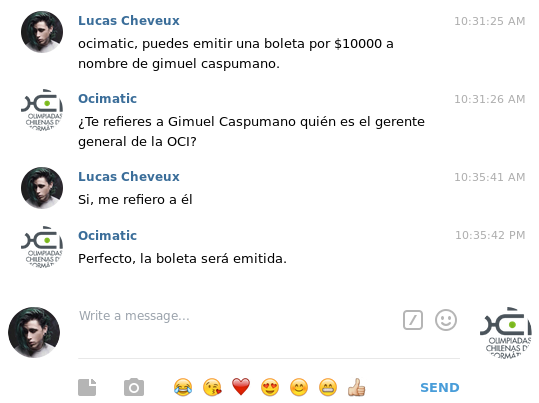
\includegraphics[scale=0.45]{ocimatic_talk2.png}}
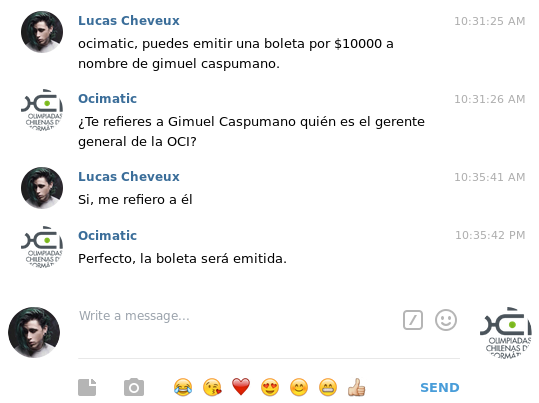
\includegraphics[scale=0.45]{ocimatic_talk2.png}
\end{center}
Ocimatic es un software extremadamente sofisticado e internamente utiliza
complejos algoritmos con el fin de procesar y entender el texto ingresado por
los usuarios.
Un algoritmo importante dentro de ocimatic está encargado del reconocimiento de
\emph{entidades}.
Para ocimatic, una entidad es cualquier fragmento de un texto que
corresponda al nombre de una persona o al de una organización.
Por ejemplo, en el texto ``\texttt{Gimuel Caspumano es el gerente general
  de la OCI.}''
se pueden reconocer dos entidades: \emph{Gimuel Caspumano} y \emph{OCI}.

Dado un texto, una entidad puede representarse con un par de números
$(a,b)$ que indican respectivamente la posición inicial y final en que la
entidad aparece en el texto.
Por ejemplo, dado el texto de ejemplo anterior la entidad \emph{Gimuel Caspumano}
puede representarse con el par (1,16) y la entidad \emph{OCI} con el par
(46,48).
Esto puede apreciarse mejor en la siguiente figura.

\begin{center}
\newcolumntype{C}{@{}>{\centering}p{0.866em}@{}}
\begin{tabu}{C|C|C|C|C|C|C|C|C|C|C|C|C|C|C|C|C|C|C|C|C|C|C|C|C|C|C|C|C|C|C|C|C|C|C|C|C|C|C|C|C|C|C|C|C|C|C|C|C}
  \taburulecolor{lightgray}
  % \hline
  \rowfont{\tiny}
  1&2&3&4&5&6&7&8&9&10&11&12&13&14&15&16&17&18&19&20&21&22&23&24&25&26&27&28&29&30&31&32&33&34&35&36&37&38&39&40&41&42&43&44&45&46&47&48&49\\
  \hline
  \rowfont{\small}
  G&i&m&u&e&l& &C&a&s&p&u&m&a&n&o& &e&s& &e&l& &g&e&r&e&n&t&e& &g&e&n&e&r&a&l&%
  &d&e& &l&a& &O&C&I&.
\end{tabu}
\end{center}

El equipo de desarrollo de ocimatic está experimentando algunos problemas con
el reconocimiento de entidades y necesitan de tu ayuda.
Específicamente, ocimatic está reconociendo algunas entidades que están
\emph{contenidas} dentro de otras.
Por ejemplo, para el texto de ejemplo anterior, ocimatic actualmente reconoce las
siguientes entidades: $(1, 6)$, $(8, 16)$, $(1, 16)$ y $(46, 48)$.
Es claro que la entidad $(1, 6)$, correspondiente al texto \emph{Gimuel}, y la
entidad $(8, 16)$, correspondiente al texto \emph{Caspumano}, están
contenidas dentro de la entidad $(1, 16)$, correspondiente al texto \emph{Gimuel
  Caspumano}.
Formalmente, decimos que una entidad $(a_1,b_1)$ está contenida dentro de una
entidad $(a_2,b_2)$ si $a_2\leq a_1$ y $b_1\leq b_2$.

La OCI está interesada en saber cuál es el impacto de este problema.
Dado un conjunto de entidades, tu tarea es evaluar el impacto contando la
cantidad de entidades que están contenidas dentro de otra.
\end{problemDescription}

\begin{inputDescription}
  La primera línea contiene un entero $N$ correspondiente al número de entidades.
  Cada una de las siguientes $N$ líneas contiene dos enteros $a$ y $b$ ($1\leq
  a\leq b \leq 10^9$) describiendo una entidad $(a,b)$.
  Se garantiza que la entrada no contiene líneas repetidas, es decir, no habrán
  dos entidades iguales.
\end{inputDescription}

\begin{outputDescription}
  La salida debe contener una única línea con un entero correspondiente a la cantidad de
  entidades que están contenidas dentro de otra.
\end{outputDescription}

\begin{scoreDescription}
  \score{15} Se probarán varios casos donde $1\leq N\leq 2$.
  \score{30} Se probarán varios casos donde $2< N \leq 100$.
  \score{35} Se probarán varios casos donde $100< N \leq 10^5$.
\end{scoreDescription}

\begin{sampleDescription}
\sampleIO{sample1}
\sampleIO{sample2}
\end{sampleDescription}

\end{document}
